\clearpage
\section{Data I/O Formats}

\subsection{Input Format} \hspace{1pt}\\

\SASfit supports a simple ASCII format. Options for reading ASCII
data can be set in the corresponding menu, where one can set an
input format and the number of lines to be skipped at the beginning
of the data file. To set an input format one has to supply a string
like "{\tt xyer}". Each line which does not contain valid float
numbers are skipped automatically. Each line further should at least
contain as many valid numbers as the supplied format string
characters. That means if the line contains only three numbers but
the format string is 4 or more characters long the line will be
ignored. Separators between numbers can be "white space",
"tabulator", or ",". For identifying the columns the characters and
their position in the string are interpreted. {\tt x}, {\tt y} and
{\tt e} stands for the scattering vector $Q$, scattering intensity
$I(Q)$ and its error $\Delta I(Q)$, respectively. {\tt r} defines
the column for a resolution parameter $\sigma$. The position of the
character in the string defines which data column is assigned to
$Q$, $I(Q)$, $\Delta I(Q)$, and $\sigma$. In case of double
occurrence of a character the position of the last one is the
significant position. Any characters not belonging to \{{\tt x},{\tt
y},{\tt e},{\tt r}\} can be used to skip a column. A definition
string need to contain
at least the two characters {\tt x} and {\tt y}. \\

\begin{description}
\item[Example 1 (HMI-BerSANS format)] ~\\
{\tiny
\begin{verbatim}
%File
FileName=D0002831.200 FileDate=28-Jun-99 FileTime=11:57:16
Type=SANSDIso Title=IMF
%Counts
 2.651E-02, 2.372E+02, 4.650E+00
 3.240E-02, 2.170E+02, 2.291E+00
 3.829E-02, 1.898E+02, 1.713E+00
 4.418E-02, 1.743E+02, 1.479E+00
 5.007E-02, 1.528E+02, 1.318E+00
 5.596E-02, 1.361E+02, 1.153E+00
\end{verbatim}
} \centerline{$\vdots$ \hspace{5cm} ~}
~\\
As the first lines start with a string, they will be automatically
ignored. To interpret the three columns as $Q$, $I(Q)$, $\Delta
I(Q)$ the format string should be simply {\tt xyz}. The HMI-BerSANS
format can also be read in by explicitly selecting instead of the
"ASCII"-format
the "HMI"-format button in the menu. \\[1cm]

\item[Example 2] \hspace{1pt}\\
{\tiny
\textcolor[rgb]{0.98,0.00,0.00}{$\mathbf{\lceil}$}
\verb"      19         0         0         0         0         0         0         6"\\
\verb"  0.100000E+01   0.100000E+04   0.000000E+00   0.100000E+01   0.120000E+01"\\
\verb"  0.000000E+00   0.000000E+00   0.000000E+00   0.000000E+00   0.000000E+00"
\textcolor[rgb]{0.98,0.00,0.00}{$\mathbf{\rfloor}$}
\begin{verbatim}
teflon              instrument tests
1  2.617993E-04   3.700000E+01   4.301163E+00
2  1.062462E-03   6.412500E+01   1.634587E+00
3  2.107973E-03   1.410135E+03   5.207492E+00
4  3.167636E-03   1.752197E+03   4.801586E+00
5  4.189463E-03   7.581771E+02   2.810281E+00
                   :
                   :
45  1.255376E-02   1.486688E+01   2.197023E-01
46  1.360724E-02   1.204012E+01   1.927716E-01
47  1.466810E-02   1.026648E+01   1.679423E-01
\end{verbatim}
}
~\\
A definition string {\tt ixye} would ignore the leading line number
at the beginning of each data line, but in the present example also
the first 3 lines would also be interpreted as data points. To skip
them one has to use the option for skipping leading lines in a data
file. In the above case the number should be set to 3 or 4. As the
4$^\text{th}$ line is anyway ignore a value of 3 is sufficient to
skip non data points.
\\[1cm]

\item[Example 3] ILL data files from regrouped treatment ({\tt gnnnnnn.eee}).\\
{\tiny
\begin{verbatim}
 Sample - d corrs    TEST prot/deutr. ellipt. chs  44 lines+(Q, I(Q), errI(Q))
  ILL  SANS D11
\end{verbatim}
\textcolor[rgb]{0.98,0.00,0.00}{$\mathbf{\lceil}$}
\verb"        8303         1        37         1        42        38"\\
\textcolor[rgb]{1.0,1.00,1.00}{$\mathbf{\lceil}$}
\verb"           14        32         0         3         1"
\textcolor[rgb]{0.98,0.00,0.00}{$\mathbf{\rfloor}$}
\begin{verbatim}
  spol 20-Oct-1995  9:16:09
   AvA1 0.0000E+00 AsA2 9.5000E-01 XvA3 1.0000E+00 XsA4 1.0000E+00 XfA5 0.0000E+00
  S...  8303  0  1.00E+00 P100 0.5% 221   Sbak  8309  0  2.00E+00 Blank523 193
  V...  8301  0  1.00E+00 Hhaps 911

    0.0000 ! Theta-0 Detector offset angle
   32.5000 ! X0 cms Beam centre
   32.5000 ! Y0 cms Beam centre
    1.0000 ! Delta-R cms regrouping step
    2.5000 ! SD m Sample-detector distance
   10.5400 ! Angstroms incident wavelength
    5.6000 ! m collimation distance
    1.0000 ! concentration
       -3. ! ISUM central window sum
        1. ! flux monitor counts
  180.0000 ! degrees detector sector width
    0.0000 ! degrees sector orientation
   10.0000 ! % wavelength spread
   20.0000 ! mm source slit width x
    0.0000 ! mm source slit height y
   10.0000 ! mm sample width x
    0.0000 ! mm sample height y
   10.0000 ! mm detector x pixel size
   10.0000 ! mm detector y pixel size
    0.0000 ! degrees sample normal/beam
    0.0000 ! K sample temperature
    0.0000 ! sample transmission
    1.0000 ! mm sample thickness
  900.0000 ! secs counting time
    0.0000 ! reserved
    0.0000 ! reserved
    0.0000 ! reserved
    0.0000 ! reserved
    0.0000 ! reserved
    0.0000 ! reserved
    0.0000 ! reserved
    0.0000 ! reserved
\end{verbatim}
\textcolor[rgb]{0.98,0.00,0.00}{$\mathbf{\lceil}$}
\verb"         37         0         0         0         0         0         0         6"\\
\textcolor[rgb]{1.0,1.00,1.00}{$\mathbf{\lceil}$}
\verb"    0.100000E+01   0.250000E+03   0.000000E+00   0.100000E+01   0.105400E+01"\\
\textcolor[rgb]{1.0,1.00,1.00}{$\mathbf{\lceil}$}
\verb"    0.000000E+00   0.000000E+00   0.000000E+00   0.000000E+00   0.000000E+00"\\
\textcolor[rgb]{1.0,1.00,1.00}{$\mathbf{\lceil}$}
\verb"0.000000E+00   0.000000E+00   0.000000E+00"
\textcolor[rgb]{0.98,0.00,0.00}{$\mathbf{\rfloor}$}
\begin{verbatim}
    2.194656E-03   3.442688E-01   8.329221E-02
    5.466116E-03   3.000000E-01   5.008947E-02
    8.480323E-03   3.877941E-01   4.232426E-02
    1.189216E-02   6.498784E-01   1.519078E-02
    1.497785E-02   7.493181E-01   1.173622E-02
\end{verbatim}
\centerline{$\vdots$ \hspace{5cm} ~} }
\noindent To read in a
regrouped ILL data file one has to use the definition string {\tt
xye} and secondly one has to skip the first 44 lines in the data
file to ignore also the lines marked with
\textcolor[rgb]{0.98,0.00,0.00}{$\mathbf{\lceil}$}
\textcolor[rgb]{0.98,0.00,0.00}{$\mathbf{\rfloor}$}. If one does not
skip the first 44 lines the marked lines are interpreted erroneously
also as data points. The other lines at the beginning of the data
file are ignored as they do not fulfill the condition that they have
3 columns containing only valid numbers.
\end{description}

\subsection{Error bar} \hspace{1pt}\\

\noindent
In case no error bar is supplied \SASfit will try to guess one.
To do this an polynomial $y_p(Q)$ of degree $p$
\begin{align}
y_p(Q) &= \sum_{k=0}^p c_k Q^k
\end{align}
is fitted to the data point $i$ and its $n^\textrm{th}$ neighbors to the left and right,
i.e. is fitted to $2n+1$ points from $I_{i-n}(Q_{i-n})$ to $I_{i+n}(Q_{i+n})$.
After the fit $\chi_i^2$ is calculated
\begin{align}
\chi_i^2&=\sum_{j=i-n}^{i+n} \left(I_j(Q_j)-y_P(Q_j)\right)^2
\end{align}
The error bar $\Delta I_i$ for $Q_i$ is than defined as
\begin{align}
\Delta I_i &= \sqrt{\frac{\chi_i^2}{2n-p}}
\end{align}
\SASfit is using two nearest neighbors $n=2$ and fitting a polynomial of \
degree $p=2$ to it to guess an error bar.
This procedure gives reasonable error bars as long as the data are oversampled and do not show sharp features within the data points $i-n$ and $i+n$. A diffraction peak or a minimum in a form factor like for monodisperse particle might not reasonable well described by the polynomial and consequently the resulting error bar will get large. Furthermore systematic errors in the absolute intensity like an overall scaling factor will not be recognized. The procedure to guess the error bar is basing on the assumption that the scattering curve behaves locally approximately like a polynomial function of degree $p=2$.

\begin{figure}[htb]
\begin{center}
\subfigure[simulated model data set with supplied error bars]{\label{fig:ModelDataWithError}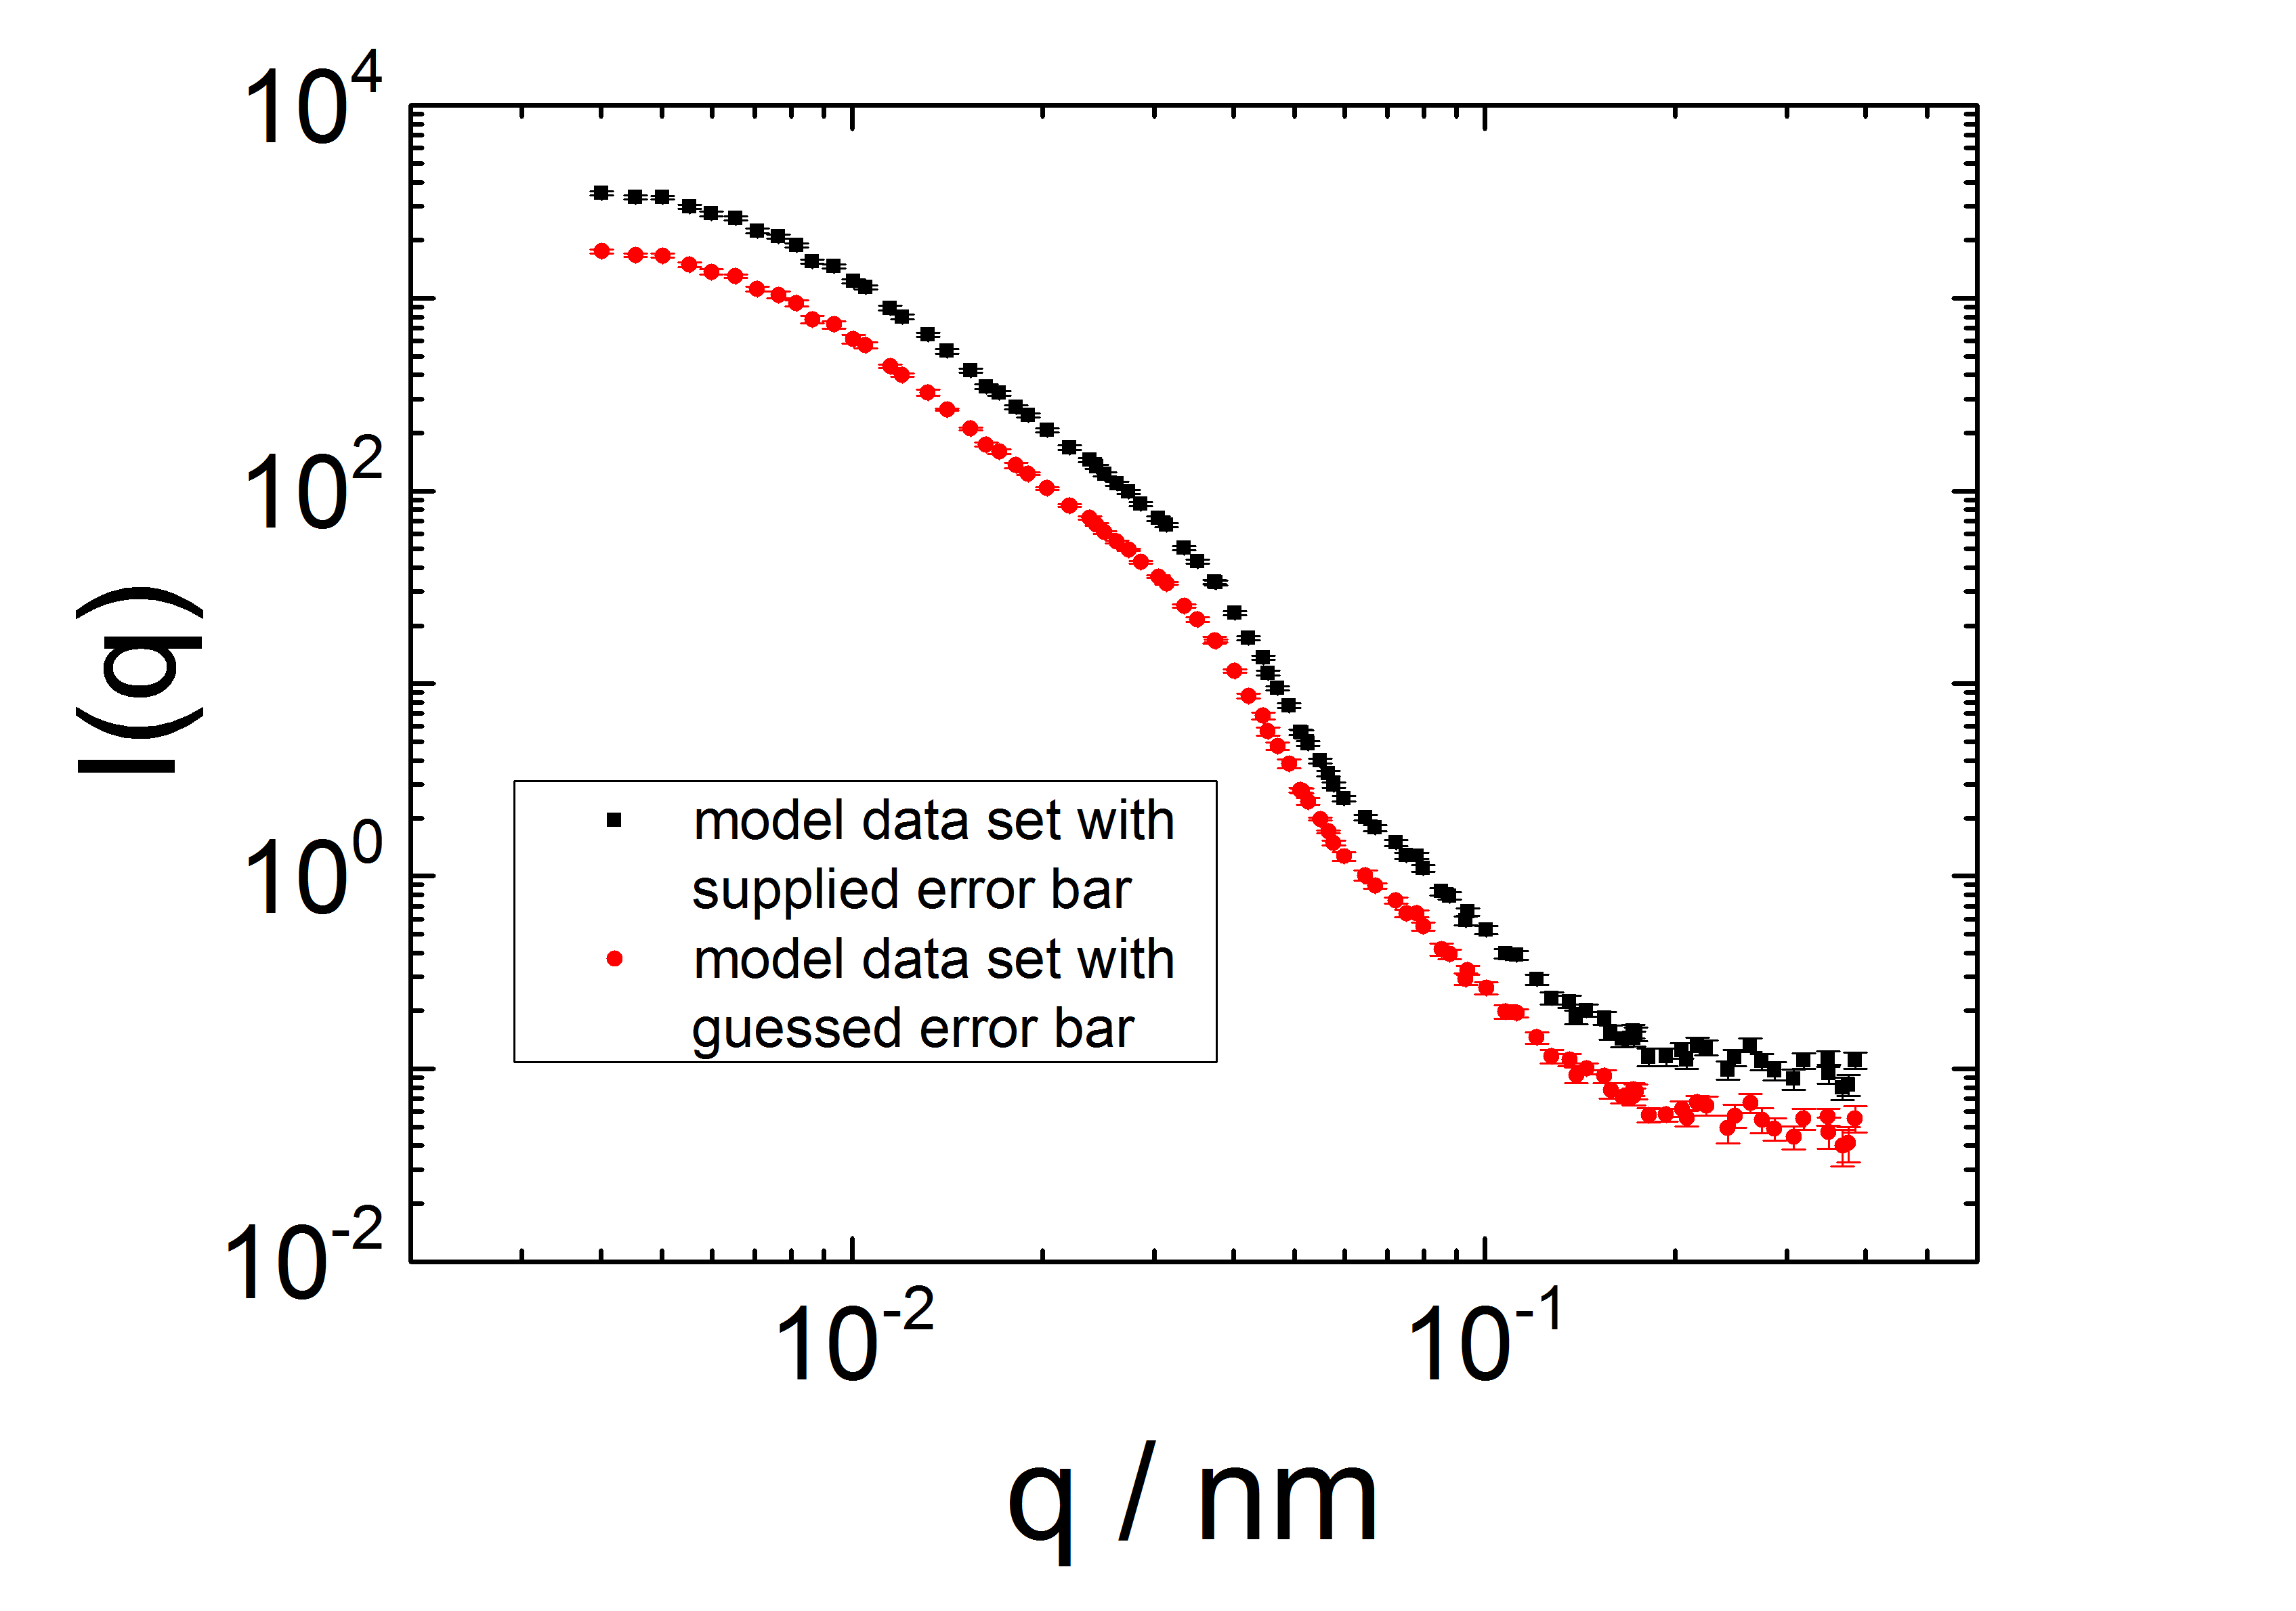
\includegraphics[width=0.47\textwidth]{../images/ErrorBar/ModelDataWithError.png}}
\subfigure[Ration between supplied error bar and the error bar guessed bz \SASfit]{\label{fig:ErrorGUI}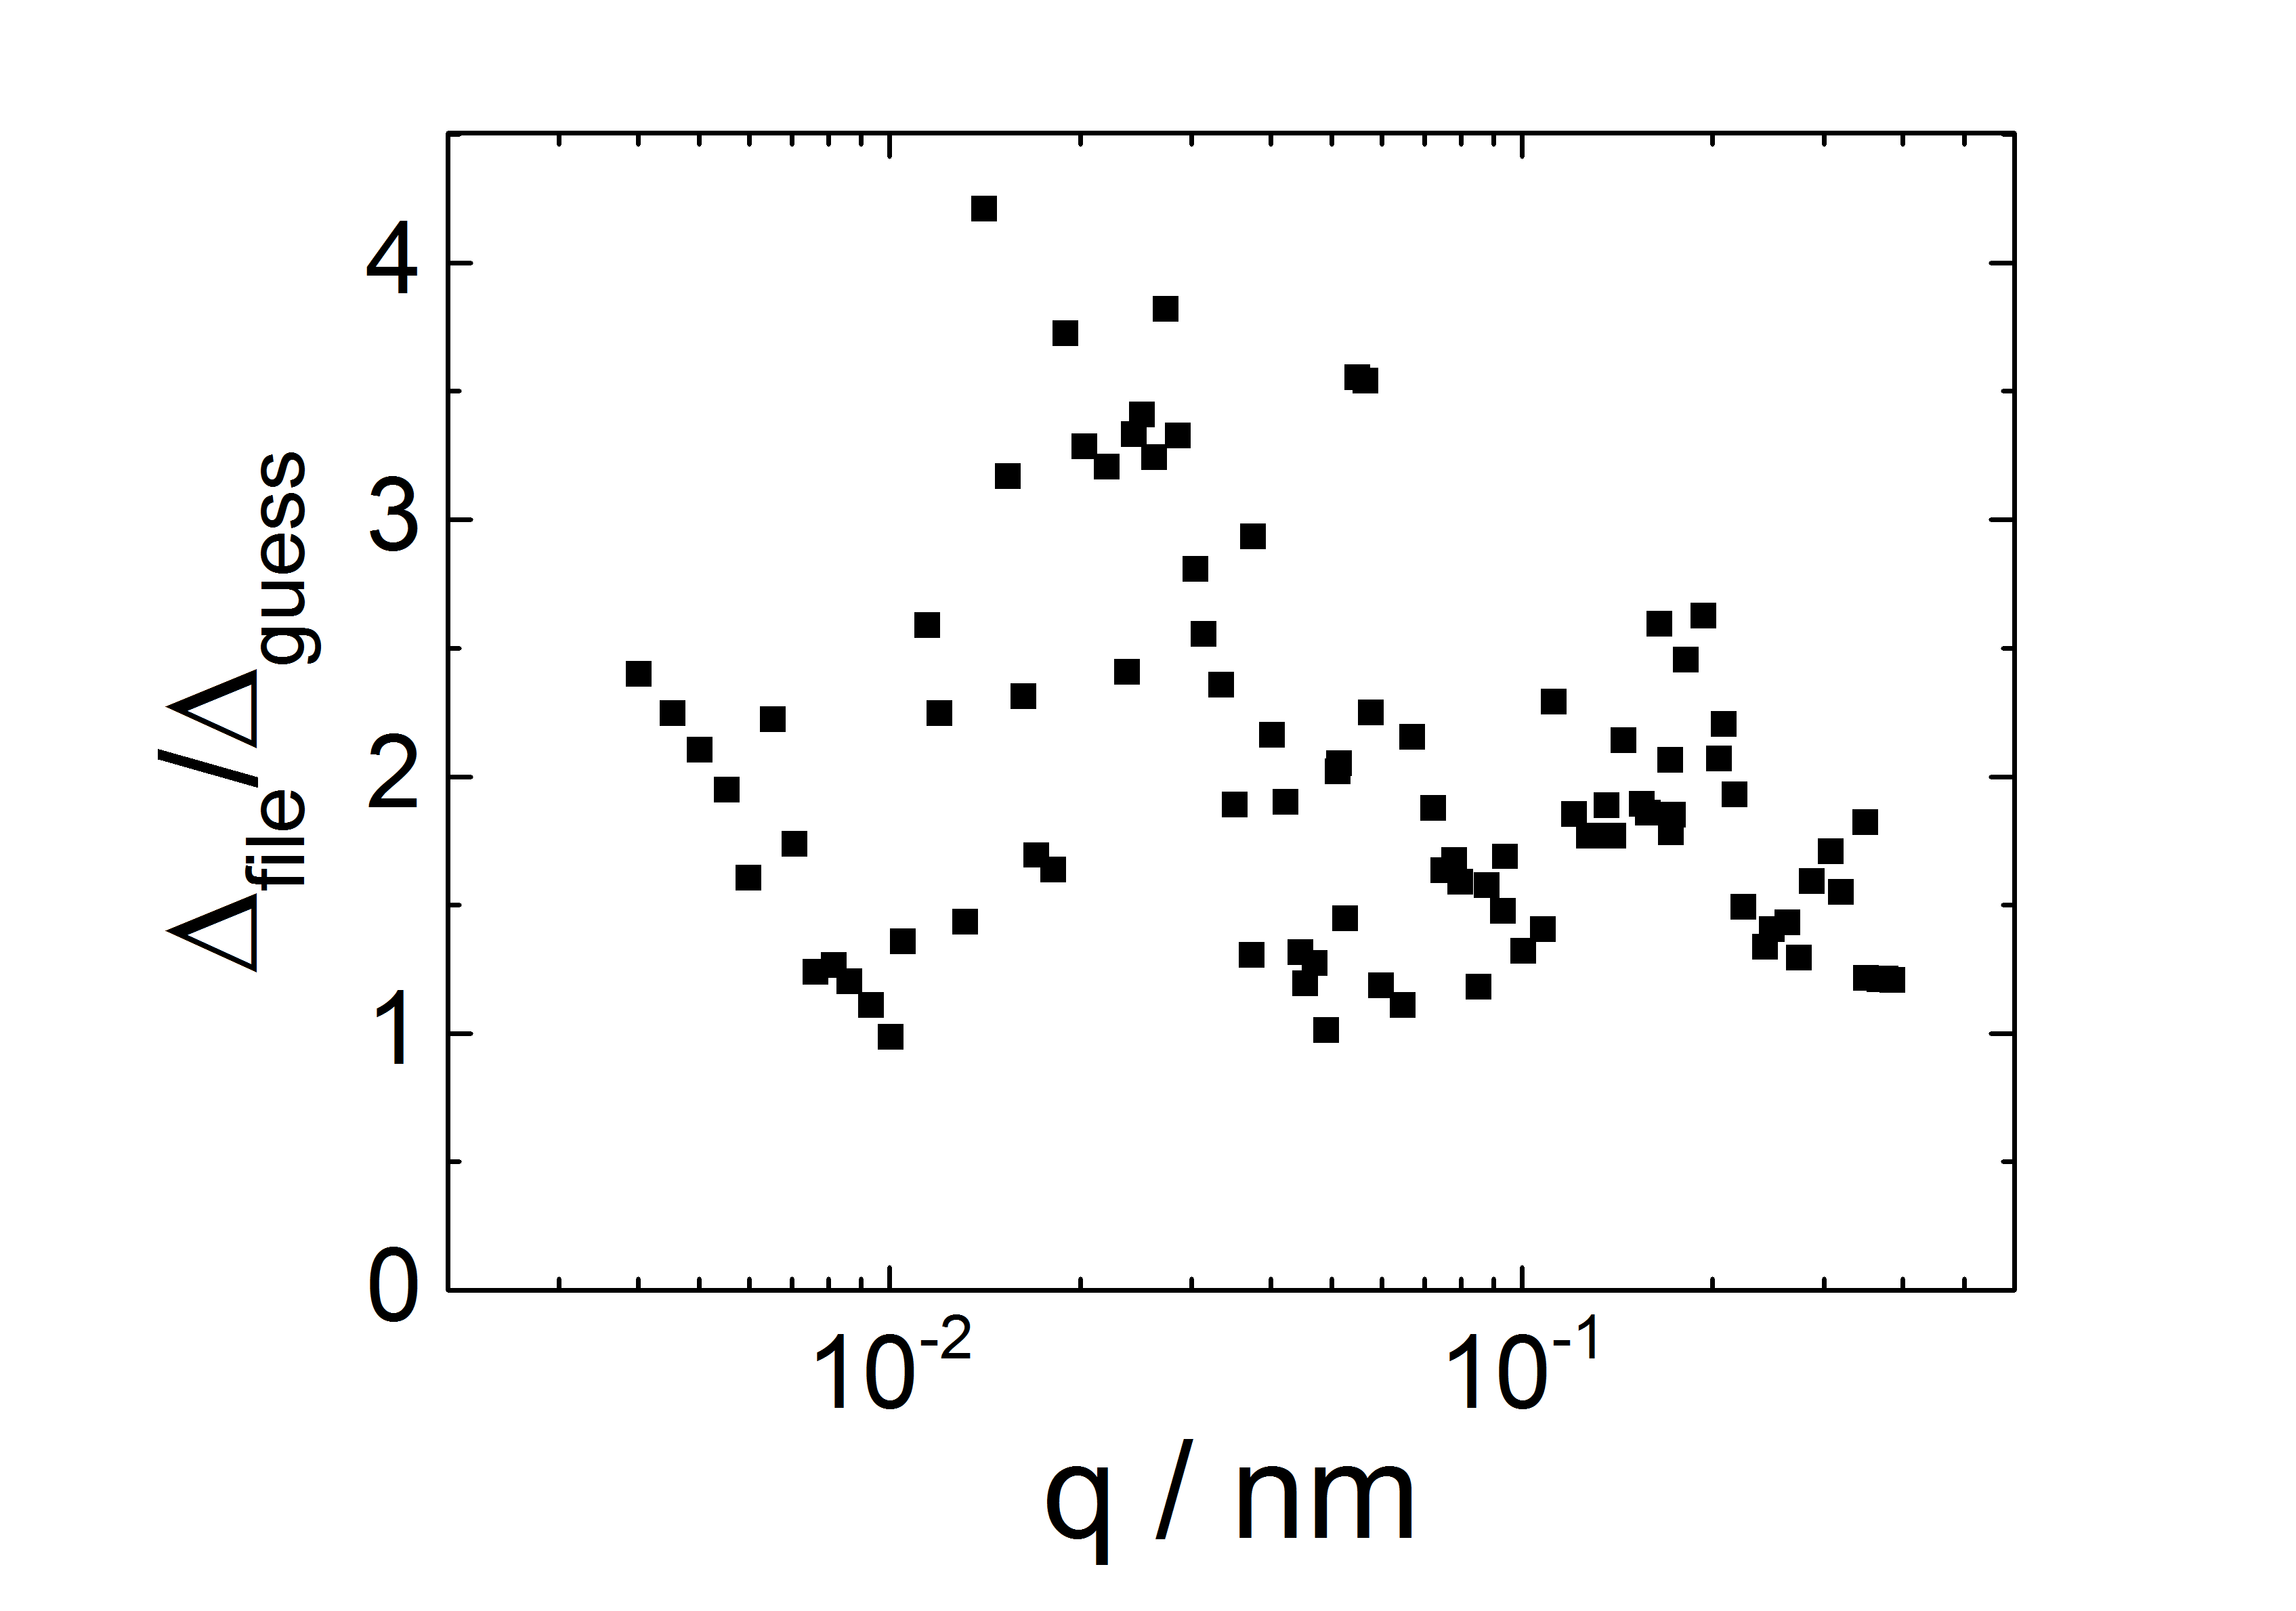
\includegraphics[width=0.47\textwidth]{../images/ErrorBar/RatioErrSuppGuess.png}}
\end{center}
\begin{center}
\subfigure[simulated model data set with supplied error bars]{\label{fig:ModelDataWithError2}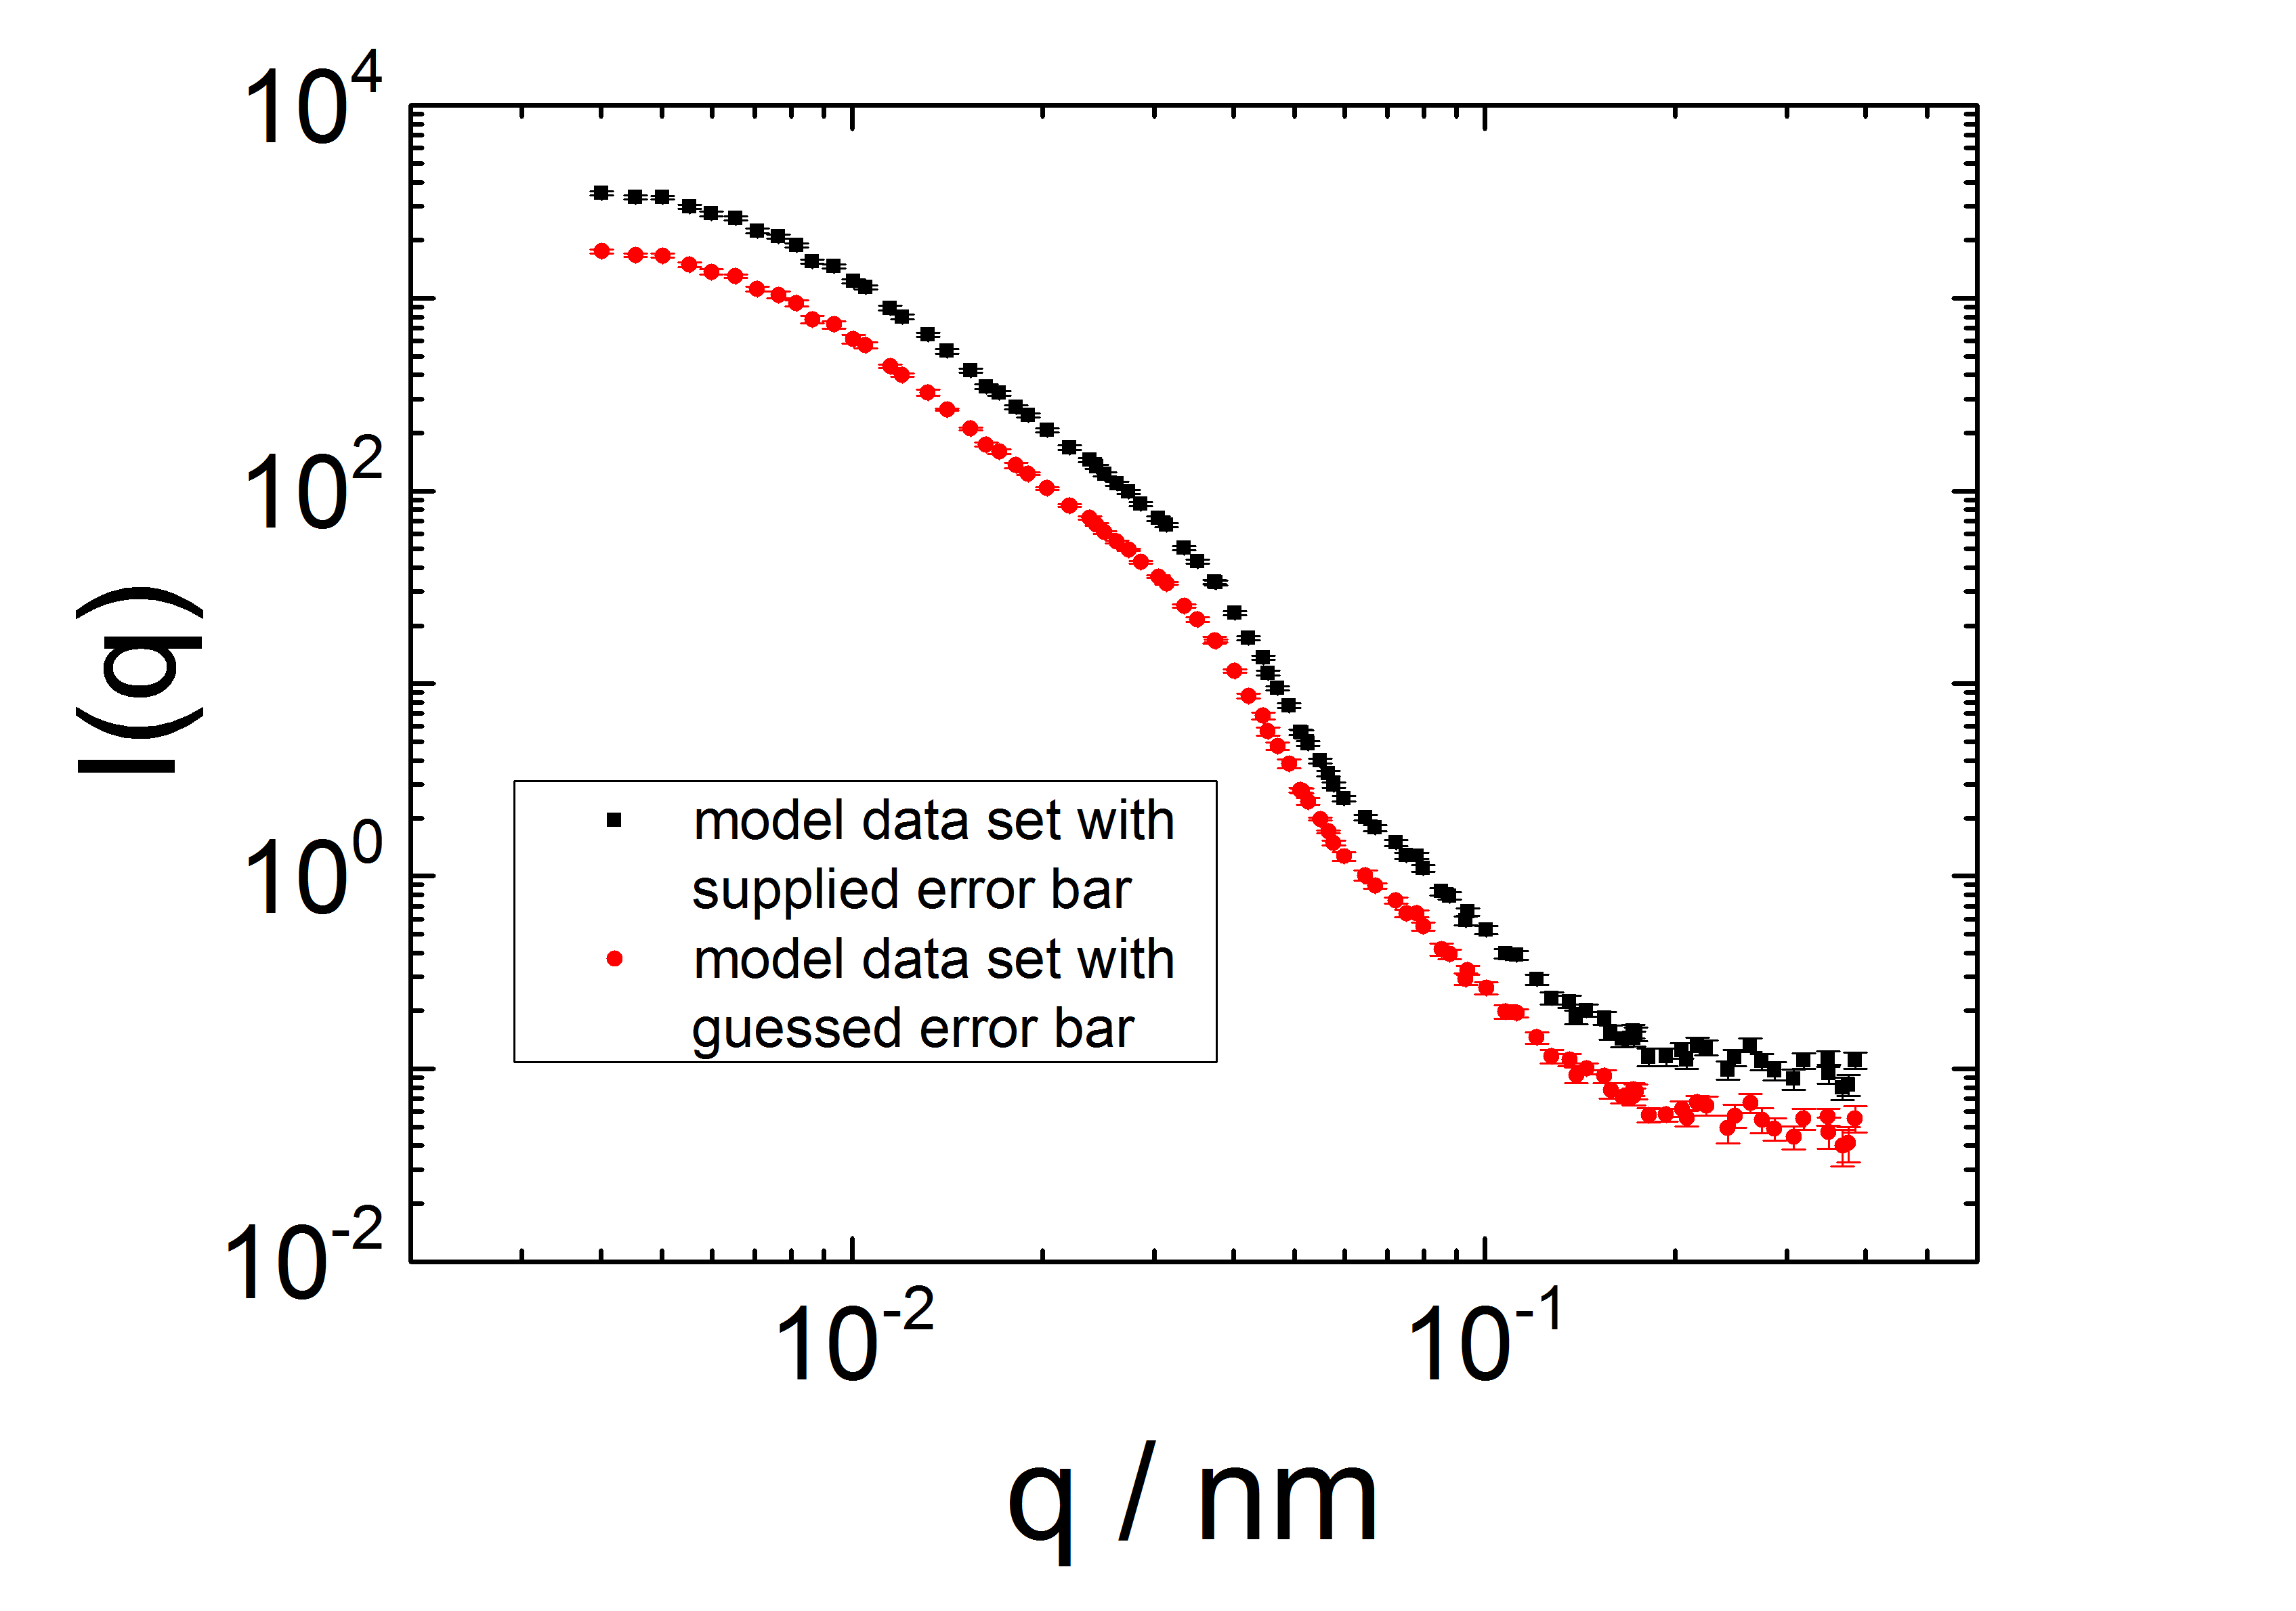
\includegraphics[width=0.47\textwidth]{../images/ErrorBar/ModelDataWithError.png}}
\subfigure[Ration between supplied error bar and the error bar guessed bz \SASfit]{\label{fig:ErrorGUI2}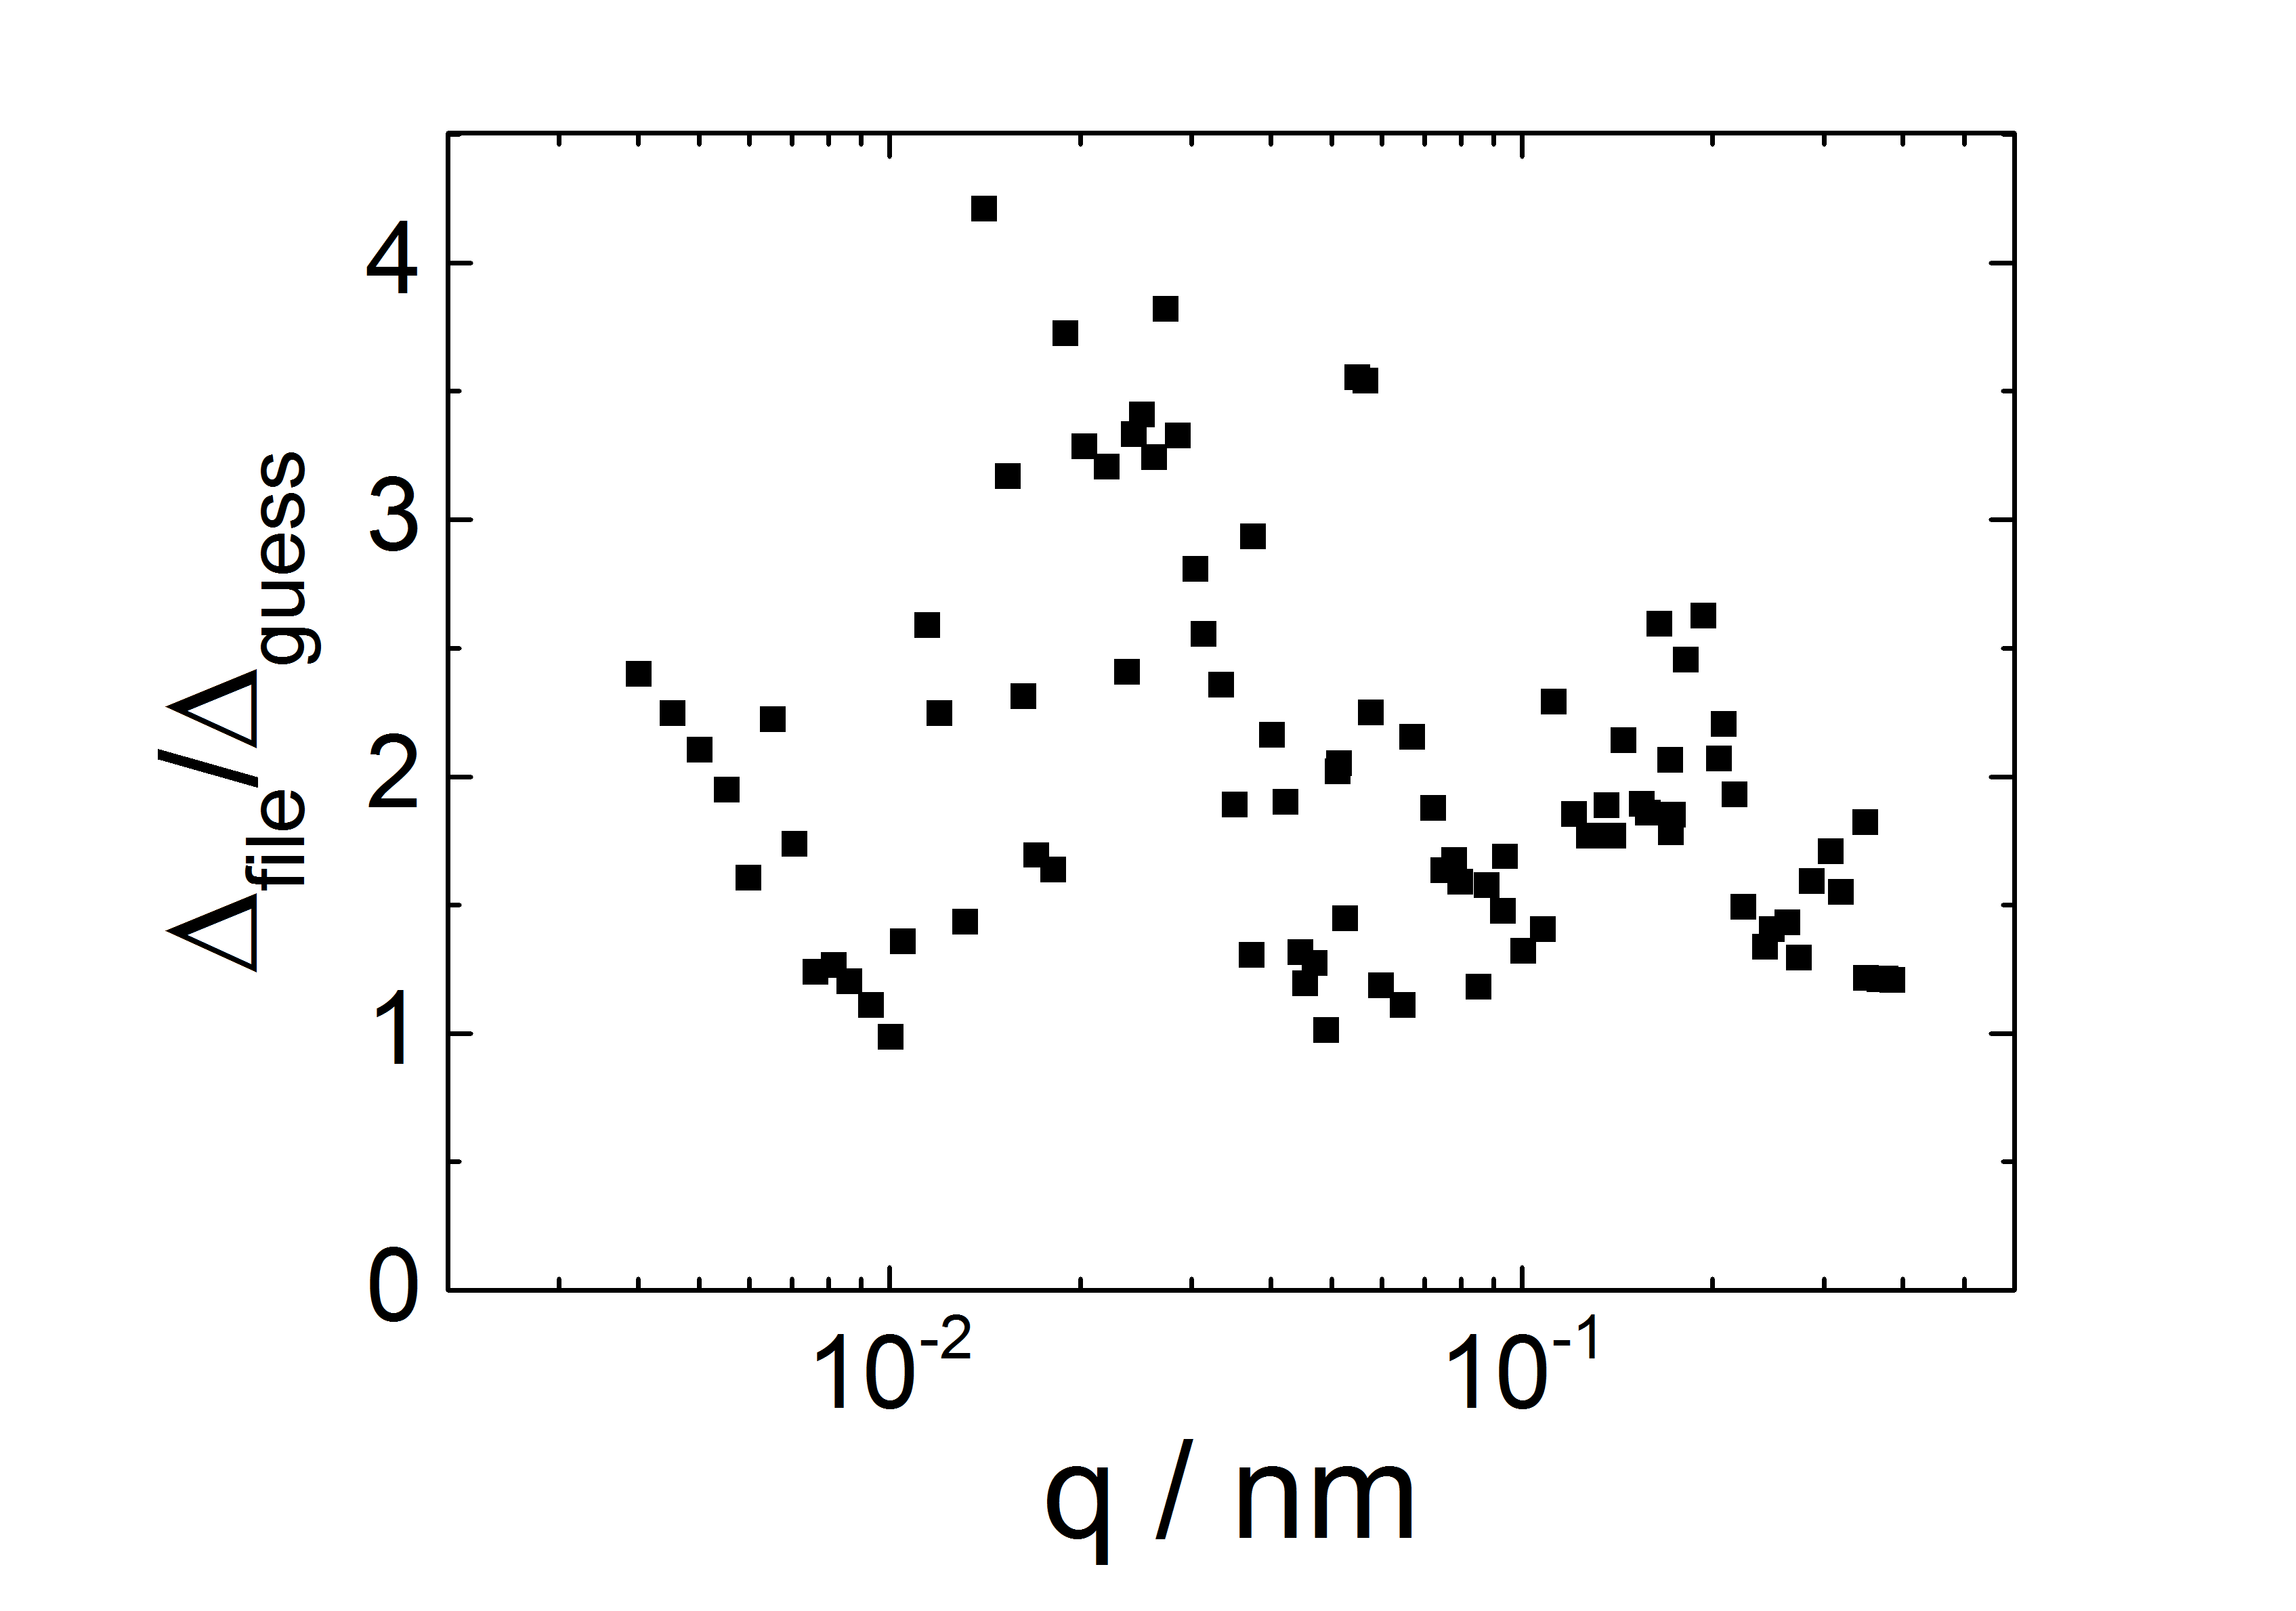
\includegraphics[width=0.47\textwidth]{../images/ErrorBar/RatioErrSuppGuess.png}}
\end{center}
\caption{Comparison of a simulated model data set with supplied error bar and an error bar guessed by \SASfit.}
\label{fig:ErrBar}
\end{figure}

\vspace{1cm}

\subsection{Export Format} \hspace{1pt}\\

\noindent
{\bf Example for an exported data file:}\\
{\tiny
\begin{verbatim}
  0.00401571,      3497.47,      90.7282,            0,   0.00401571,       260294,           -1,            0,
  0.00454087,         3340,      84.9531,            0,   0.00454087,       254548,           -1,            0,
   0.0050096,      3322.47,      79.6313,            0,    0.0050096,       248833,           -1,            0,
  0.00552335,      2983.23,      73.7254,            0,   0.00552335,       241949,           -1,            0,
  0.00598495,      2737.17,      68.4395,            0,   0.00598495,       235226,           -1,            0,
   0.0065309,      2598.76,      62.3109,            0,    0.0065309,       226647,           -1,            0,
  0.00706977,       2233.9,      56.4829,            0,   0.00706977,       217551,           -1,            0,
  0.00764207,      2080.96,      50.6186,            0,   0.00764207,       207264,           -1,            0,
  0.00815988,      1882.88,      45.6557,            0,   0.00815988,       197459,           -1,            0,
\end{verbatim}
\centerline{$\vdots$ \hspace{5cm} $\vdots$}
\begin{verbatim}
            ,             ,             ,             ,    0.0445634,      1535.14,           -1,            0,
            ,             ,             ,             ,    0.0453557,      1473.71,           -1,            0,
            ,             ,             ,             ,    0.0470219,      1340.34,           -1,            0,
            ,             ,             ,             ,    0.0490017,      1192.64,           -1,            0,
            ,             ,             ,             ,    0.0510837,      1055.44,           -1,            0,
\end{verbatim}
} If one like to export the data of an $xy$-plot all curves are
stored in a single data file. Each curve will occupy four columns
($Q$, $I(Q)$, $\Delta I(Q)$, $\sigma$). If an error $\Delta I(Q)$ is
not available, e.g. for theoretical data curves, the corresponding
column will be filled with -1. Similar is valid for the resolution
parameter $\sigma$ which will be set to 0 in case it is not
available. The individual columns are separated by ",". If the curve
have different amount of data points the column will be filled with
empty space for the missing data. This comma separated data format
has been chosen as it can be imported easily by many commercial
plotting softwares. The drawback of this format is, however, that
\SASfit cannot read it correctly, if the individual curves are of
different length.
